\documentclass{beamer}
%
% Choose how your presentation looks.
%
% For more themes, color themes and font themes, see:
% http://deic.uab.es/~iblanes/beamer_gallery/index_by_theme.html
%
\mode<presentation>
{
  \usetheme{default}      % or try Darmstadt, Madrid, Warsaw, ...
  \usecolortheme{default} % or try albatross, beaver, crane, ...
  \usefonttheme{default}  % or try serif, structurebold, ...
  \setbeamertemplate{navigation symbols}{}
  \setbeamertemplate{caption}[numbered]
} 

\usepackage[english]{babel}
\usepackage[utf8x]{inputenc}

\title[Data Mining]{Visualization-D3.js}
\author{Bingyu Wang}
\institute{Northeastern University}
\date{July 28, 2014}

\begin{document}

\begin{frame}
  \titlepage
\end{frame}

% Uncomment these lines for an automatically generated outline.
%\begin{frame}{Outline}
%  \tableofcontents
%\end{frame}

\section{Introduction}

\begin{frame}{Introduction}

\begin{itemize}
  \item Why d3.js? 
  \item Getting started
  \item Summary
\end{itemize}

\end{frame}

\section{d3.js}

\subsection{Intro to d3.js}

\begin{frame}{Why d3.js?}

\begin{itemize}
	\item Most graphing packages take a configuration object.
	\item D3 is much more flexible and direct, and gets over the fact that the option you want are never available.
	\item Slower to get started but much more productive and flexible. 
	\item Great documentation, examples community.
\end{itemize}

% Commands to include a figure:
%\begin{figure}
%\includegraphics[width=\textwidth]{your-figure's-file-name}
%\caption{\label{fig:your-figure}Caption goes here.}
%\end{figure}

%\begin{table}
%\centering
%\begin{tabular}{l|r}
%Item & Quantity \\\hline
%Widgets & 42 \\
%Gadgets & 13
%\end{tabular}
%\caption{\label{tab:widgets}An example table.}
%\end{table}

\end{frame}

\begin{frame}{Fundamentals} 
Working with D3 requires an appreciation of the following concepts:

\begin{itemize}
	\item HTML 
	\item DOM
	\item CSS
	\item JavaScript
	\item SVG
\end{itemize}
\end{frame}

\begin{frame}{HTML}
Hypertext Markup Language is used to structure content for web browsers. The simplest HTML page looks like this:
\begin{figure}
\centering
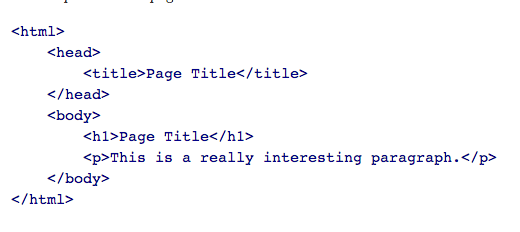
\includegraphics[width=1.0\textwidth]{./images/HTML.png}
\caption{\label{fig:samplemax} HTML}
\end{figure}
\end{frame}

\begin{frame}{DOM}
The Document Object Model refers to the hierarchical structure of HTML. Each bracketed tag is an element, and we refer to elements' relative relationships to each other in human terms: parent, child, sibling, ancestor, and descendant. In the HTML above, body is the parent element to both of its children, h1 and p (which are siblings to each other). All elements on the page are descendants of html.
\end{frame}

\begin{frame}{DOM Example} 
\begin{figure}
\centering
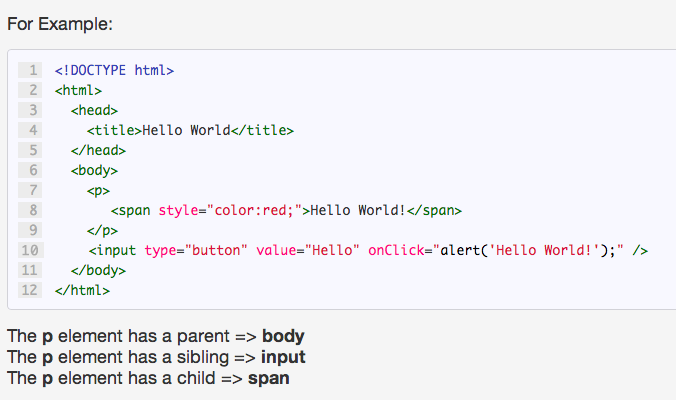
\includegraphics[width=1.0\textwidth]{./images/DOM.png}
\caption{\label{fig:DOM} DOM}
\end{figure}
\end{frame}

\begin{frame}{CSS}
Cascading Style Sheets are used to style the visual presentation of HTML pages.
\newline \\
D3 uses CSS-style selectors to identify elements on which to operate, so it is important to understand how to use them.
\end{frame}

\begin{frame}{JavaScript}
JavaScript is a dynamic scripting language that can instruct the browser to make changes to a page after it has already loaded.
\end{frame}

\begin{frame}{SVG}
D3 is at its best when rendering visuals as Scalable Vector Graphics. SVG is a text-based image format. Meaning, you can specify what an SVG image should look like by writing simple markup code, sort of like HTML tags. For example:
\begin{figure}
\centering
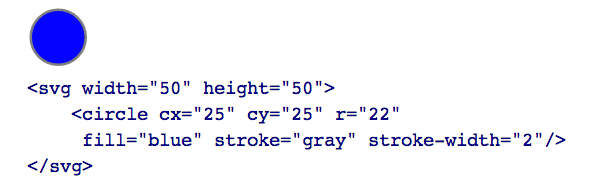
\includegraphics[width=1.0\textwidth]{./images/SVG.png}
\caption{\label{fig:samplemax} SVG}
\end{figure}

\end{frame}


\begin{frame}{Getting Started}
\begin{enumerate}
	\item Adding elements
	\item Binding data
	\item Using data
	\item Drawing div
	\item Drawing SVG
\end{enumerate}
\end{frame}

\begin{frame}{Adding elements}
An example: \textbf{d3.select("body").append("p").text("New paragraph!");} \\
Let us walk through what just happened. In sequence, we:
\begin{enumerate}
	\item Invoked D3's select method, which selects a single element from the DOM using CSS selector syntax. (We selected the body.)
	\item Created a new p element and appended that to the end of our selection.
	\item Set the text content of that new, empty paragraph to New paragraph!
\end{enumerate} 
\end{frame}

\begin{frame}{Binding data}
Data visualization is a process of mapping data to visuals. Data in, visual properties out. \\
With D3, we bind our data input values to elements in the DOM. Binding is like attaching or associating data to specific elements, so that later you can reference those values to apply mapping rules.
\end{frame}

\begin{frame}{Data}
D3 is smart about handling different kinds of data, so it will accept practically any array of numbers, strings, or objects(themselves containing other arrays or key/value pair). It can handle \textbf{JSON} (and \textbf{GeoJSON}) gracefully, and even has a built-in method to help you load in \textbf{CSV} files. 
For example:
\begin{figure}
\centering
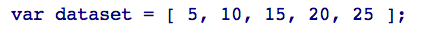
\includegraphics[width=1.0\textwidth]{./images/Data.png}
\caption{\label{fig:data} Data}
\end{figure}
\end{frame}

\begin{frame}{Using Data}
We use .data(datatset) for loading data. Once it is loaded. We can use High-functioning to parse each element in the whole dataset. For example:
\begin{figure}
\centering
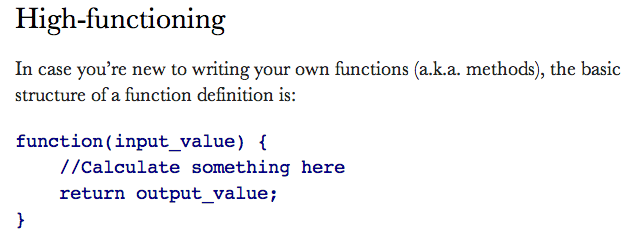
\includegraphics[width=1.0\textwidth]{./images/High_function.png}
\caption{\label{fig:high} High Function}
\end{figure}
\end{frame}

\begin{frame}{Drawing divs}
This is for starting drawing with data. Define a \textbf{div} as following:
\begin{figure}
\centering
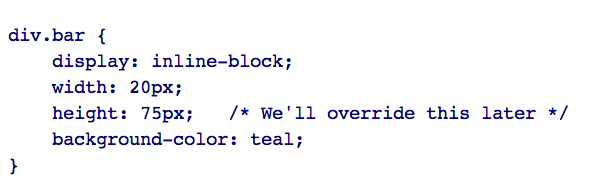
\includegraphics[width=1.0\textwidth]{./images/DIV.png}
\caption{\label{fig:div} DIV}
\end{figure}
\end{frame}

\begin{frame}{Drawing divs}
The next step is using the div we just defined, named \textbf{bar}. The following is the example:
\begin{figure}
\centering
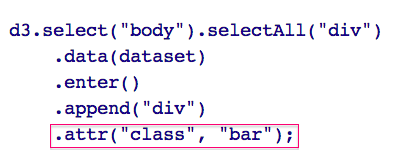
\includegraphics[width=1.0\textwidth]{./images/BAR.png}
\caption{\label{fig:bar} Using bar DIV}
\end{figure}
\end{frame}

\begin{frame}{Drawing divs}
The final step we want to apply our dataset = [5,10,15,20,25] to the bar's heights. Using as following:
\begin{figure}
\centering
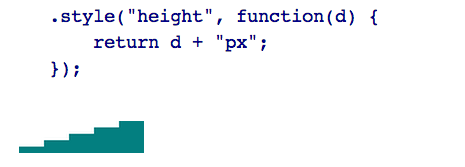
\includegraphics[width=1.0\textwidth]{./images/style.png}
\caption{\label{fig:style} Using Style}
\end{figure}
\end{frame}

\begin{frame}{SVG} 
Drawing with divs and other native HTML elements is possible, but a bit clunky and subject to the usual inconsistencies across different browsers. \\
In fact D3 is most useful when used to generate and manipulate visuals as SVGs. Using SVG is more \textbf{reliable, visually consistent, and faster}.
\end{frame} 

\begin{frame}{SVG Shapes} 
There are a number of visual elements that you can include between those SVG tags, including:
\begin{itemize}
	\item rect 
	\item circle
	\item ellipse 
	\item line
	\item text
	\item path
\end{itemize}
\end{frame}

\begin{frame}{SVG Shapes Examples} 
\begin{figure}
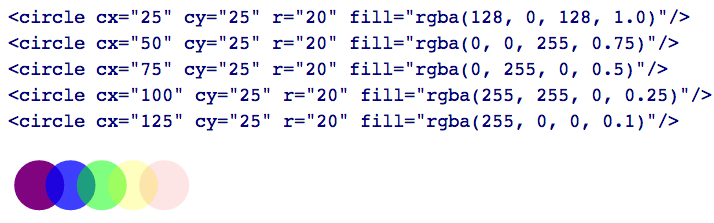
\includegraphics[width=1.0\textwidth]{./images/SVG_example.png}
\caption{\label{fig:svgexample} SVG Example}
\end{figure}
\end{frame}

\begin{frame}{Drawing SVGs}
Now if we are familiar with the basic structure of an SVG image and its elements, how can we start generating shapes from our data? \\
We noticed that all properties of SVG elements are specified as attributes. That is, they are included as property/value pairs within each element tag, like this: 
\begin{figure}

\includegraphics[width=1.0\textwidth]{./images/svg_property.png}
\caption{\label{fig:svgproperty} SVG Property}
\end{figure}
Fortunately, we have already used D3's handy \textbf{append()} and \textbf{attr()} methods to create new HTML elements and set their attributes. We can use these methods to generate SVG images. 
\end{frame}

\begin{frame} {Drawing SVGs}
Two steps to use the data set generate SVG images. 
\begin{enumerate}
	\item Create the SVG
	\item Data-driven Shapes 
\end{enumerate}
\end{frame}

\begin{frame}{Create the SVG}
First, we need to create the SVG element in which to place all our shapes. Example as following:
\begin{figure}
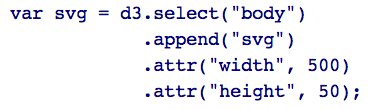
\includegraphics[width=1.0\textwidth]{./images/create_SVG.png}
\caption{\label{fig:svgcreate} Create a SVG}
\end{figure}
\end{frame}

\begin{frame} {Data-driven Shapes}
Time to add some shapes. Still use \textbf{var dataset = [5,10,15,20,25]}.\\
Then use data() to iterate through each data point, creating a circle for each one, as following:
\begin{figure}
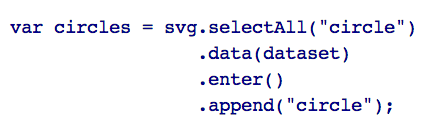
\includegraphics[width=1.0\textwidth]{./images/svg_circles.png}
\caption{\label{fig:svgcircles} Creating Circles on SVG}
\end{figure}
\end{frame}

\begin{frame} {Data-driven Shapes}
Look at the code in previous slide, 
\begin{enumerate}
	\item selectAll() will return empty references to all circles(which don't exist yet)
	\item data() binds our data to the elements we're about to create
	\item enter() returns a placeholder reference to the new element
	\item  append() finally adds a circle to the DOM
\end{enumerate}
\end{frame}

\begin{frame}{Data-driven Shapes}
To continue play with circles in SVG. All these circles still need positions and sizes. Like:
\begin{figure}
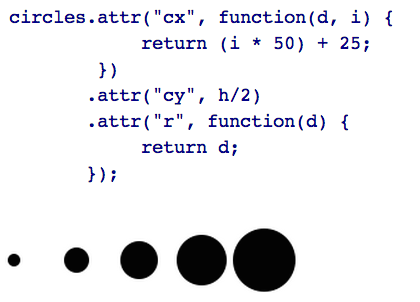
\includegraphics[width=1.0\textwidth]{./images/circles.png}
\caption{\label{fig:circles} Circles}
\end{figure}
\end{frame}

\begin{frame}{Data-driven Shapes}
Do more color fills and strokes. Like:
\begin{figure}
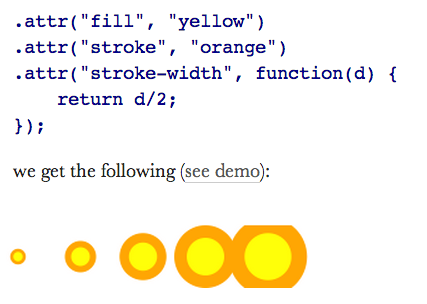
\includegraphics[width=1.0\textwidth]{./images/color_circles.png}
\caption{\label{fig:colorcircles} Color Circles}
\end{figure}

\end{frame}

\subsection{Summary}

\begin{frame}{Summary} 
This is the basics we have learned so far:
\begin{itemize}
	\item Make DOM objects, attach data to them, use CSS.
	\item The data can affect any attribute, shape, color, size, position, opacity, text, etc.
	\item All the attributes can have transitions applied. 
\end{itemize}
\end{frame}

\begin{frame}
There is more stuff to help us:
\begin{itemize}
	\item Add and remove objects to dynamically update visualization.
	\item Helper functions for different charts: chord, histogram, hierarchy, pie, stack, tree, cluster, etc.
	\item Drag and touch events, date formatting etc.
\end{itemize}
\end{frame}

\begin{frame}{References}
\begin{itemize}
	\item http://alignedleft.com/ 
	\item http://lws.node3.org/
	\item https://www.dashingd3js.com/
	\item http://d3js.org/
\end{itemize}
\end{frame}

\end{document}
